\documentclass[9pt,oneside]{amsart}
\usepackage{url}
\usepackage{cancel}
\usepackage{xspace}
\usepackage{graphicx}
\usepackage{multicol}
\usepackage{subfig}
\usepackage{amsmath}
\usepackage{amssymb}
\usepackage[a4paper,width=170mm,top=18mm,bottom=22mm,includeheadfoot]{geometry}
\usepackage{booktabs}
\usepackage{array}
\usepackage{verbatim}
\usepackage{caption}
\usepackage{natbib}
\usepackage{float}
\usepackage{pdflscape}
\usepackage{mathtools}
\usepackage[usenames,dvipsnames]{xcolor}
\usepackage{afterpage}
\usepackage{tikz}
\usepackage[utf8]{inputenc}
\usepackage{csquotes}
\usepackage{amsmath}

\newcommand{\hcancel}[1]{
    \tikz[baseline=(tocancel.base)]{
        \node[inner sep=0pt,outer sep=0pt] (tocancel) {#1};
        \draw[black] (tocancel.south west) -- (tocancel.north east);
    }
}

\definecolor{lightyellow}{rgb}{1,0.98,0.9}
\definecolor{lightblue}{rgb}{0.9,0.9,0.98}
\definecolor{lightpink}{rgb}{1,0.94,0.95}

\definecolor{initial}{rgb}{.7,0.0,0.0}
\definecolor{reviewed}{rgb}{0.0,0.0,0.7}

\providecommand{\todo}[1]{{\color{initial}#1}}
\providecommand{\review}[1]{{\color{reviewed}#1}}

\newcommand{\firsthomesteadblock}{\ensuremath{\mathit{TBA}}}

\DeclarePairedDelimiter{\ceil}{\lceil}{\rceil}
\newcommand*\eg{e.g.\@\xspace}
\newcommand*\Eg{e.g.\@\xspace}
\newcommand*\ie{i.e.\@\xspace}

\title{On Issues Arising With Blockchain Voting \\ {\smaller \today}}
\author{
    Alexander Schoedon
}
\author{
    Robert David McLeod
}
\author{
    Johannes Ponader
}
\begin{document}

\pagecolor{lightblue}

\begin{abstract}
\enquote{The digital revolution remains marginal in the field of decision-making, and is almost completely absent of our political institutions. Trust in our political systems require more frequent votes, votes that have greater impact, votes that are not made out of paper. Because voting is at the roots of democratic societies, e-voting should be flawless. Users don't only chose who or what they vote for, they chose how they will do it.} --- \textit{nemos.io} % TODO REMOVE OR CITE
\end{abstract}

\maketitle

\setlength{\columnsep}{20pt}
\begin{multicols}{2}

\section{Digital Revolution}\label{sec:motivation}

% the digital revolution remains marginal in the field of decision-making, and is almost completely absent of our political institutions [MARGOT-DUCLOT~2015]
% trust in our political systems require more frequent votes, votes that have greater impact, votes that are not made out of paper [MARGOT-DUCLOT~2015]
% because voting is at the roots of democratic societies, e-voting should be flawless [MARGOT-DUCLOT~2015]
% users don't only chose who or what they vote for, they chose how they will do it [MARGOT-DUCLOT~2015]

\enquote{Everything that can be decentralized, will be decentralized.} -- \textit{Johnston's Law} [JOHNSTON~et~al.~2013].\par
Distributed ledgers have the potential to disrupt the way society works. Not only the banking or the financial technology sector is affected by this new technology called \textit{blockchain} but almost everything from the internet of decenthings to distributed governance.\par
Regarding the focus of this paper, blockchain has the potential to revolutionize voting, direct and liquid democracy approaches. The idea is to decentralize democratic processes, promote election fairness and online voting security [VARSHNEYA~et~al.~2015].\par
Known electronic voting systems are usually proprietary and centralized, e.g., a single entity controls everything: the hardware, the code base, the data base, system outputs and even the monitoring tools [NOIZAT~2014]. Adam Kaleb Ernest of the \textsc{Follow My Vote} project describes the electronic voting process in the United States as \textit{black box voting} and links the lack of transparency directly to lower voter turnouts [ERNEST~2014]. In addition, the used systems have been vulnerable for software and hardware attacks for a long time. Sufficient alternatives still have to be developed [VARSHNEYA~et~al.~2015].\par
It's about time to talk about 21st centurary approaches to voting: technology which will be decentralized and legislation which will be distributed to pave the way for a modern society [ROCKWELL~2014].

\section{On blockchain voting}
Will blockchain create the base technology for democratic applications? The answer is still outstanding. A lot of questions arise regarding both the voting process and the underlying technology. A lot of them remain unanswered. This paper tries to ask all questions and -- where possible -- gather and evaluate potential approaches to solve them.

\subsection{Why blockchain matters}
After Satoshi Nakamoto presented the first concept of a fully decentralized and trustless currency \textsc{Bitcoin (BTC)} in 2008 [NAKAMOTO~2008] and published the first blockchain protocol reference implementation in 2009, many years have passed until the underlying technology seriously got recognized as a game changer by the technology scene. Blockchain tools today are considered and valued with a high potential. The current emerge of blockchain related start-ups aswell as global operating coorperations entering the market is often compared to the beginning of the internet [ÉPIÉ~et~al.~2015].\par
The impact on society, industry and governance hardly can be estimated. Suddenly, transactions can share information without any middle man. The blockchain is owned, run  and monitored by everyone, but controlled by anyone [ÉPIÉ~et~al.~2015].\par
The non-hierarchical, self-organizing, peer-to-peer collaboration nature of blockchain ecosystems within communitarian network structures is the foundation for both censorship resistance and full transparency, which leaves no room for any tampering. This is a big feature that nothing but blockchains can provide [SCOTT~2016] [KAYE~2016].

\subsection{Blockchain 2.0 technology}
In 2013 so called \textit{Bitcoin 2.0} projects or \textit{blockchain 2.0} technologies emerged. They aim is to provide collectively maintained decentralized ledgers that record things other than currency transactions and store all manner of diverse data, including voting decisions [SCOTT~2016].\par
At the cutting edge of the scene are smart contracts, small scripts on the blockchain, which participants can interact with. The new contract-orientated development paradigm allows for a switch in terminology: the \textit{trustless} nature of transactions on the blockchain moves aside for \textit{trust-enabling} transparent scripts doing exactly as programmed [SCOTT~2016].\par
% smart contracts: automatically execute the conditions and terms [ÉPIÉ~et~al.~2015]
% virtual, autonomous, without central control, trustable [ÉPIÉ~et~al.~2015]
Among the most innovative blockchain 2.0 technologies of the recent years are \textsc{Bitshares (BTS)}, \textsc{Ripple (XRP)}, \textsc{Nxt (NXT)} and \textsc{Ethereum (ETH)}.\par % @TODO Stellar, Tendermint, Hyperledger
Bitshares offers a stack of financial services including exchange and banking on a blockchain. It is mainly trageted at next-level financial applications and developed the concept of decentralized autonomous coorperations (\textsc{DAC}) which operate autonomous on the blockchain, issue tokes and payout shareholders as programmed.\par
Ripple is a commercial solution for the financial technology sector. Its distributed financial technology allows for banks to directly transact with each other without the need for a central counterparty or correspondent.\par
% @TODO check for relevance Stellar, Tendermint, Hyperledger
Nxt improves the financial technology, crowdfunding and governance industries by providing powerful, modular toolsets to build any application on top of the blockchain.\par
Blockchain 2.0 projects are often considered to pave the way for the \textit{Web 3.0} which will be decentralized. Ethereum claims to be \enquote{the way the internet was supposed to work}. \enquote{What Bitcoin does for payments, Ethereum does for anything that can be programmed.}, states Grace Caffyn from Coindesk referring to the underlying technology.\par
%\begin{figure}[H]
%\centering
%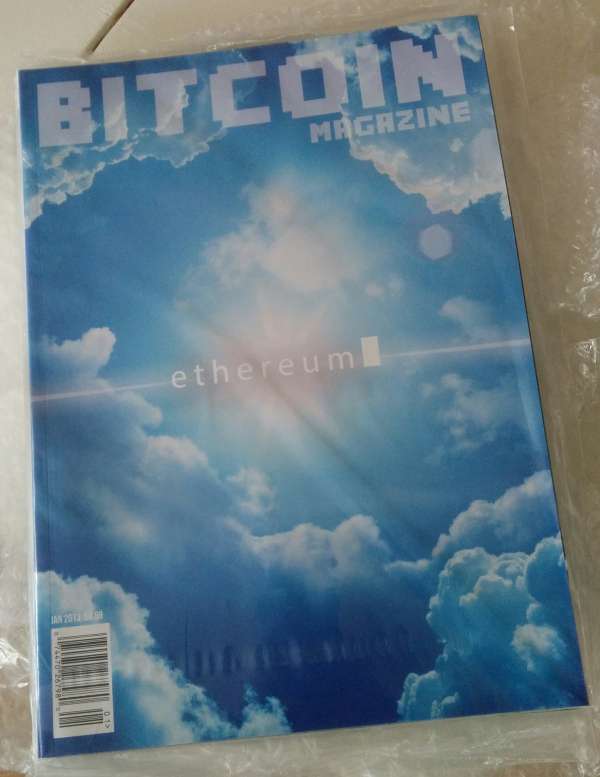
\includegraphics[draft,width=0.3\textwidth]{bitmag.png}
%\caption{The Bitcoin Magazine January 2014 Issue: On Ethereum.}
%\label{fig:mag}
%\end{figure}
The Ethereum blockchain contains a distributed virtual machine (\textsc{EVM}) which enables code on the blockchain to be executed. Whereas every blockchain technology offers it's own, often limited scripting languages, the revolutionary concept behind the EVM is the lifting of all limits by implementing a \textit{turing-complete} programming language. This allows -- in theory -- to build everything on top of the Ethereum blockchain technology: Smart contracts implement the logic, the blockchain manages the decentralized consensus and users can interact with trustable decentralized applications (\textsc{DApps}) [ÉPIÉ~et~al.~2015].

\subsection{Blockchain voting versus \enquote*{votechains}}
Voting is a key functionality of blockchain technology. The underlying consensus protocols on most distritubted peer-to-peer solutions always have to include ways to update protocols and restore consensus upon disputes. A prominent example is the Bitcoin Improvement Proposal \#BIP34, of the crypto-currency \textsc{Bitcoin} [NAKAMOTO~2008], proposing miner behaviour on softforking mechanics. This is voting on a very technical level and not considered part of this paper.\par
The following projects and voting references rather focus on applications or services \textit{on top of} blockchains, enabling democratic participation in any kind of groups, communities or societies.

\subsection{Requirements for voting applications}
\label{sec:req}
Electronic or online voting has to follow the same high standards as traditional paper or offline voting processes do. Necessary key feauteres and requirements will be gathered below. Existing approaches to blockchain based voting applications will be checked against these criteria.\par
How can elections be auditable and anonymous? How can a voter's identity be private but verifiable? [VARSHNEYA~et~al.~2015] aswell as [ERNEST~2016] and [BORGSTRUP~2014] define following key features for blockchain voting.
\begin{itemize}
\item \textbf{Fair}. Participants can vote for anyone they like, not only the candidate they prefer most.
\item \textbf{Accessible}. Everyone should be able to use it without the introduction of any entry barriers.
\item \textbf{Anonymous}. Privacy of voters has to be protected and it should be infeasable to determine identity behind a vote. % @TODO sybil
\item \textbf{Authenticated}. The identity on the blockchain must be unique, and provable certified to vote to ensure only registered voters can take part in elections.
\item \textbf{Secure}. It also has to be impossible to decrypt voter's identities or to link voter's to voting behaviour. All communications should be encrypted.
\item \textbf{Integer}. It should not be possible to tamper with votes.
\item \textbf{Coercion-resistant}. The system should be able to prevent coercion of voters to vote in a certain way.
\item \textbf{Verifiable}. Individuals must be able to verify their votes are included in the final tally. Also, anyone must be able to check the election results were computed correctly.
\item \textbf{Auditable}. The whole process must enable a complete audit trail from the first user authentication through the final election.
\item \textbf{Decentralized}. A trust-enabling and tamper-resistant blockchain voting system has to be decentralized by design.
\item \textbf{Open source}. It has to be possible to examine code and to verify everything works as proposed.
\end{itemize}
Only applications fullfilling all points above should be considered for official electronic voting processes. % TODO OPEN SOURCE: Proposed solutions which fail to deliver open source products will be automatically applied a zero score as they are impossible to peer review.

\section{Evaluation of exisiting implementations}

\subsection{Projects utilizing blockchain voting}
Below is a short overview of existing research, organizations and implementations of blockchain based democracy applications.


\subsubsection{Follow My Vote}
Formerly \enquote*{Vote DAC}, Follow My Vote is a distributed autonomous company (\textsc{DAC}) emerged from the Bitshares community. It's currenlty heavily developing both a stake-weighted and a one-person-one-vote (\textsc{1p1v}) blockchain voting DAC by a team around Adam Kaleb Ernest [ERNEST~2016].\par
This is currently the most advanced project on creating a next generation voting platform. It utilizes the Bitshares blockchain with it's delegated proof-of-stake (\textsc{DPOS}) consensus mechanisms. The Vote DAC implements an end-to-end verified voting system which enables verified users to take part in transparent but private polls [ERNEST~2014].\par
An exact technical protocol specification is outstanding [VARSHNEYA~et~al.~2015] and can not be evaluated at the time of writing. Questions remain on why the whole project is designed as a coorporation which issues shares (10 billion VOTE tokens) [ERNEST~2014]. It might be a way to raise funds but having shares in a coorporation which allows voting by stake raises new issues: The most power has the user with the biggest stake.\par
In addition, the voter registration is onymous and depending on a centralized voter certification authority [VARSHNEYA~et~al.~2015]. However, blind signatures allow for maximum voting privacy on the blockchain [HOURT~2015B].\par
Checking against the requirements from section \ref{sec:req}, Follow My Vote scores 10/11 points for being fair, accessible, anonymous, authenticated, secure, integer, coercion resistant, verifiable, auditable and open source.

\subsubsection{Bitmessage Vote}
In~2014 Jesper Borgstrup wrote a master's thesis on \enquote*{Private, trustless and decentralized message consensus and voting schemes} [BORGSTRUP~2014]. The protocol uses blockchain-technology and invertible bloom lookup tables for defining deadlines and timestamping of messages. Linkable ring signatures provide a scheme suitable for signing votes. A reference implementatoin is based on the PyBitmessage applicatoin.\par
He proposed a protocol to conduct anonymous, trustless, decentralized elections on the internet and mainly solved the decentralized deadline consensus issue by utilizing the Bitcoin blockchain technology to record timestamps. Multiple votes from the same voter are discarded. For elections, a list of public keys of registered voters has to exist in any form. Linkable ring signatures are used to ensure every vote comes from registered voters, the identity of voter can not be determined and double votes are easy detectable [BORGSTRUP~2014].\par
This implementation introduced issues regarding scalability. Only 8,000 voters can be registered per ballot which requires up to 2 GiB disk space. To vote, the bitmessage protocol requires a proof-of-work verification which takes up to two minutes per vote and increases in time with the number of voters. In addition, this implementation does not provide any solutions on voter authentication and the way lists of public keys are generated.\par
Checking against the requirements from section \ref{sec:req}, Bitmessage Vote scores 6/11 points for being anonymous, secure, integer, verifiable, decentralized and open source.

\subsubsection{Unchain Voting}
One of the earliest blockchain voting implementations is Unchain Voting. It's build on top of the Bitcoin blockchain. Each electronic vote is a transaction and each voter recieves voting credits -- around 0.01 BTC -- to spend them on candidate recipients. Candidates generate Bitcoin vanity addresses to be easily recognizable. Organizers of the election distribute keys to the voters. The keys are hierarchical deterministic (HD) and each voter gets one key [NOIZAT~2014].\par
Checking against the requirements from section \ref{sec:req}, Unchain Voting scores 6/11 points for being authenticated, secure, integer, verifiable, auditable and open source.

\subsubsection{Public Votes}
\label{sec:pubv}
Public Votes is an Ethereum voting application designed and implemented by Dominik Schiener. Both his proposal [SCHIENER~2015A] and more recent analytics[SCHIENER~2015B] are highlighting advantages and issues arising with Ethereum and blockchain voting.\par
The implementation utilizes a MeteorJS frontend, a MongoDB server backend and the Ethereum blockchain. It is provably fair, transparent and easy to use but should only be regarded as a proof-of-concept implementation since it is no decentralized application [SCHIENER~2015A].\par
The centralized backend is used to generate transactions and pay for the fees. In addition, the voting results will not only be stored in the Ethereum blockchain but in the MongoDB backend, to improve the overall website performance. The public record of the poll and the votes is an Ethereum smart contract on the blockchain written in Solidity [SCHIENER~2015A].\par
Flaws of this system are obvious. It is not decentralized by design, implements an IP based user \enquote*{authentication} which can be easily tampered with and the contract is not sybil attack proof as it could accept transactions from anywhere [SCHIENER~2015B].\par
Checking against the requirements from section \ref{sec:req}, Public Votes scores 5/11 points for being accessible, anonymous, secure, integer and open source.

\subsubsection{Nemos}
Developed by France's netparty, Nemos is a blockchain-proved decision making tool based on Ethereum with eleminated gas costs [MARGOT-DUCLOT~2015]. % TODO

% use blockchain tech to pave the way for new forms of political deliberation [MARGOT-DUCLOT~2015]
% nemos is a set of smart contracts to create an automated administrative framework [MARGOT-DUCLOT~2015]
% vote on anything political leaders, local decisions, legal documents, or other smart contracts [MARGOT-DUCLOT~2015]
% the first self-adapting distributed voting system [MARGOT-DUCLOT~2015]
% changes will be implemented immidiately [MARGOT-DUCLOT~2015]
% deploy new contracts automatically [MARGOT-DUCLOT~2015]
% users are contracts signed by members of the network and legally enforcable [MARGOT-DUCLOT~2015]
% nemos integrates encrypted id to register citizens not users [MARGOT-DUCLOT~2015]
% can produce hard law, legal value [MARGOT-DUCLOT~2015]
% traditionally, digital security, vote secrecy and transparency are mutually exclusive [MARGOT-DUCLOT~2015]
% blockchain elections provide strong answer to these three [MARGOT-DUCLOT~2015]

\subsubsection{Blockchain Apparatus}
The Blockchain Apparatus aims to become a blockchain-secured voting machine.

\subsubsection{Quadratic Voting $(V)^2$}
$(V)^2$ emerged from the Ether.camp hackathon in~december~2015 and developed a quadratic voting dapp based on the Ethereum network.


\subsubsection{BitVote}
BitVote suggests to be an Ethereum decentralized application (DApp) using encryption chains and a peer-to-peer hybrid technology for the purpose of proposal collaboration, information sharing and voting. There is a whitepaper draft available which was not completed in the recent two years [BALE~2014]. The reference implementation is far from complete and lacks a working blockchain integration.\par
Checking against the requirements from section \ref{sec:req}, BitVote scores 0/11 points since neither the code nor the whitepaper can be evaluated due to the lack of the most basic content.

% bitvote vs bitvit [BALE~2014]
% vote with life time [BALE~2014]
% bits units of information, vits units of voting time [BALE~2014]
% 1 vit is 1 second in a life of a voter [BALE~2014]
% stop sopa internet blackout: 20 million users, 24 hours = 480 million vit-hours expressed against sopa (18th jan 2012) [BALE~2014]
% collect and record vits in decentralized universal ledger (ethereum) [BALE~2014]
% synchronized turing tests to catch sybil accounts [BALE~2014]

\subsubsection{E-Vox}
% ukraine-based applications for voting/decision making [KONASHEVYCH~2016]
% primaries and other political processes [KONASHEVYCH~2016]
% e-petitions, local electronic plebiscites, electronic referendums [KONASHEVYCH~2016]
% voting for local councils/parliaments [KONASHEVYCH~2016]
% developed on blockchain by ambisafe/vareger group [KONASHEVYCH~2016]
% blockchain transactions carrie voting decision [KONASHEVYCH~2016]
% signed with digital signature legally recognaized in the ukraine [KONASHEVYCH~2016]
% implementing multiple e-democracy projects [KONASHEVYCH~2016]
% test case in vyshhorod [KONASHEVYCH~2016]

\subsubsection{VoteFlux}
% neutral voting block, australia (localized solution)
% no absolute control over the voting system [KAYE~2014]
% run on a distributed public network [KAYE~2014]
% able to be verified by everyone, everywhere, constantly, and consistently [KAYE~2014]
% bitcoin blockchain because security is magnitudes better than next best [KAYE~2016]
% proof of identity via electoral roll (lists the names and addresses of everyone who’s registered to vote) [KAYE~2016]
% protocol involves tokens minted by issue, able to be transfered. basic income style underlying token that doesnt expire with each issue, and has constant inflation, provides liquidity between vote tokens and anti spam measures, standard units are points as in percentage, not discreete units, "political points" [KAYE~2016]
% flux requires 1 trx per 10 minutes, using a merkele tree and ipfs [KAYE~2016]
% everything is done by OP_RETURN txs and byte strings [KAYE~2016]
% liquid democracy, moved to get-swap-vote [KAYE~2016]
% identity checked against australian electoral commision roll [KAYE~2016]
% all people who are empowered recieve N*1000000 (1M to keep it within integer maths) [KAYE~2016]
% using the blockchain just to commit data
% purely using it for the security properties, as much as possible is offchain

\subsubsection{BitCongress}
BitCongress claims to be a decentralized voting platform but is lacking references or source code, a whitepaper is available though. It proposes to use the Bitcoin blockchain for it's proof-of-work security, \textsc{Counterparty (XCP)} assets for crowdfunding and Ethereum contracts for unknown reasons [ROCKWELL~2014].\par
This is not sybil attack proof as anyone can register to become a voter and introduces issues with 3 blockchain dependencies by design. In addition, votes can be traded like any other token and could be easily shared or sold [VARSHNEYA~et~al.~2015].\par
The initial XCP crowdsale never happened in two years and this project is therefore to be considered dead. It can not be checked against the requirements in section \ref{sec:req} and scores 0/11.

\subsubsection{Democracy Earth}
Democracy.earth is a follow-up project by Santiago Siri and Pia Mancini from DemocracyOS who relocated to the United States recently. The project is currently creating a community, recruiting enthusiasts and researching on blockchain voting and identity. No possible solutions have been published yet [MANCINI~et~al.~2015].\par
DemocracyOS is a centralized web-application from Argentina which allows you to propose, debate and vote online. The team discussed blockchain integration back in~2015 twice [DEMOCRACYOS~2015A][DEMOCRACYOS~2015B]. An article on Newschallange contains first mockups which appear to use the Bitcoin blockchain for simple voting transactions [MANCINI~2015].\par
Not much more can be found and therefore, it can not be checked against the requirements in section \ref{sec:req} and scores 0/11.

\subsubsection{SureVoting}
Students from the West Virginia University WVU, Ricky Kirkendall and Ankur Kumar, are currently creating SureVoting, a student government voting app for iPads. There is no concept or code released yet though [COYNE~2015]. It can not be checked against the requirements in section \ref{sec:req} and scores 0/11.

\subsubsection{VoteCoin}
Votecoin is a proposal for a hash based voting technology. The whitepaper calls for a fair, transparent, practical solution but fails to deliver conceptual details or a working implementation [LEVEL~2014]. It can not be checked against the requirements in section \ref{sec:req} and scores 0/11.

\subsubsection{Agora Voting}
AgoraVoting had the idea to add a distributed voting system on top their working solutions [ELVIRA~2013] but failed to raise the required development funds. Due to the lack of specification and implementation, it can not be checked against the requirements in section \ref{sec:req} and scores 0/11.

\subsubsection{V-Initiative}
V-Initiative proposed a decentralized voting app but the project seems dead since the website is partially unreachable. It therefore can not be checked against the requirements in section \ref{sec:req} and scores 0/11.

\subsection{Scope for Votesapp}
The team for Votesapp wants to provide a blueprint for a better democratic process and develop blockchain based tools which educate, inform, support the decision making. This paper is initialized by them and tries to connect the projects above by promoting an improved cross-initiatives collaboration.

\section{General outline on key issues}
Currently existing solutions are not robust enough to supplement current voting schemes. Most of them incur technical cost to understand crypto-currencies, are riddled with implementation issues and vulnaribilities or lack of decentralized idenitity proof [VARSHNEYA~et~al.~2015].\par
The following chapter will focus on open issues arising with blockchain based electronic voting systems.

\subsection{Blockchain identity issue}
%\begin{figure}[H]
%\centering
%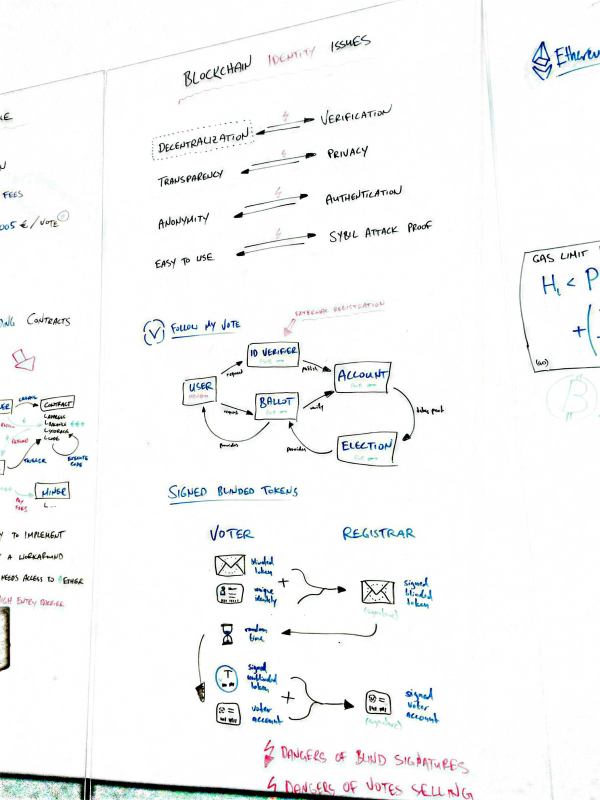
\includegraphics[draft,width=0.3\textwidth]{ident.png}
%\caption{ident.}
%\label{fig:ident}
%\end{figure}
% central authority against sybil attacks (trade off?)
% voter registration: signed blinded tokens [IMG: VOTER-REGISTRAR-BLINDED-TOKENS] [HOURT~2015A]

\subsection{Architecture considerations}
%\begin{figure}[H]
%\centering
%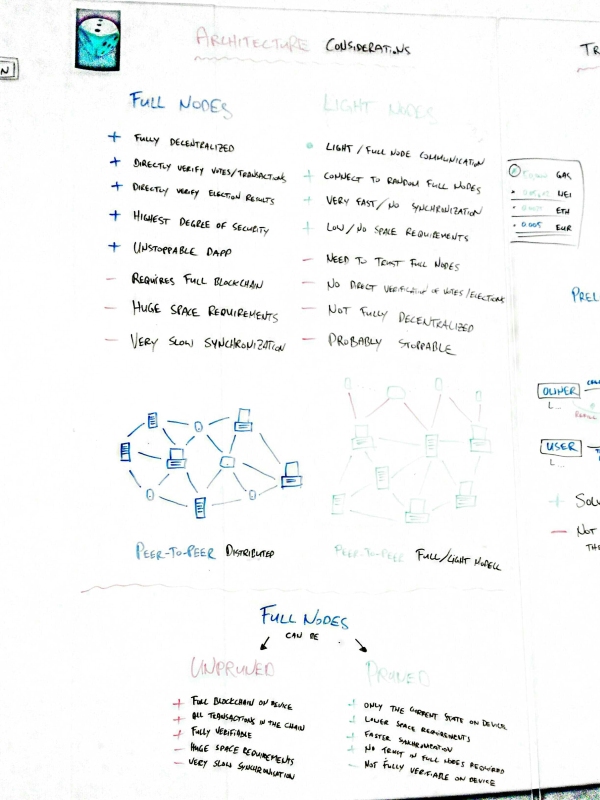
\includegraphics[draft,width=0.3\textwidth]{arch.png}
%\caption{arch.}
%\label{fig:arch}
%\end{figure}
For reference, the Bitcoin blockchain size is -- at the time of writing -- 63 GiB in size and growing at a rate of around 3 GiB per month. The Ethereum blockchain is 12 GiB in size and groing at a rate of 1.5 GiB per month.\par
This introduces a logistic, technical entry barrier for users of blockchain technology. The trade-off in decentralized, transparent and trustless systems is that every participant in the network stores its own copy of all available data.\par
Considering the \textit{inclusion} of every citizen in the world or a specific nation in a blockchain voting process, one has to consider the different levels of both technological understanding of each person -- regardless of age, education, social and cultural background -- and access to technology supporting distributed ledgers. Idially, any device from smartwatches, through smartphones, notebooks or workstations should be able to participate in the blockchain voting process. But storing a full copy of an underlying blockchain is not always possible.
\subsubsection{Light clients} % TODO IMAGE
A possible solution is the utilization of light nodes on small devices which connect to random full nodes on more dedicated devices. Full nodes store a copy the blockchain and are equal peers in the peer-to-peer network. They offer the highest degree of security as they can directly verify transactions, votes and election results. A network of full nodes directly connected to each other reaches the highest degree of decentralization and it's almost impossible to shut down or disrupt the network. Downsides of full nodes are the hugh space requirements for storing the full copy of the ledger and the very slow syncrhonization and verification process.\par
Introducing a light-to-full-node communication can bypass the synchronization issues and disk space requirements. This can be done by connecting to random full nodes in the network via any kind of API which offers querying the blockchain on such clients. The disadvantage of such an architecture is the need of trust towards the full nodes as they could deliver tampered data. The light clients can not directly verify transactions, votes and elections as they have no copy of the blockchain to calculate own results. This is a drawback in decentralization. By disrupting the communication between light and full clients or by setting up malicious full nodes, this system introduces serious vulnarabilies.
\subsubsection{State-trie pruning}
Ethereum adds another option to this considerations. Since Ethereum clients not only store the blockchain but the full state trie, it is possible to \textit{prune} the blockchain state history and save up to 80\% of the disk space. The default synchronization process is \textit{unpruned}. This stores the full blockchain on the device, verifies all block's proof-of-work and commits all transactions to update the state trie. This allows the client to verify any state of the blockchain in the past by querying recent states. The downside is -- as discussed earlier -- that this method has huge space requirements and a very slow syncrhonization process. An alternative is to prune the state trie. This only downloads the blockchain and verifies the proof-of-work but it does not commit all transactions included in the blocks. The whole state history is not calculated. After the blockchain was downloaded, the client requests the latest state from other nodes and saves it.\par
State-trie-pruning nodes might be the way to go as in most cases only the current state is interesting for the clients. This lowers space requirements and speeds up blockchain synchronization without introducing a gap of trust between nodes as seen with light client architectures. The only downside is the lack of the full state trie \textit{history}.
% @TODO BIGCHAIN DB

\subsection{Blockchain voting scalability}
%\begin{figure}[H]
%\centering
%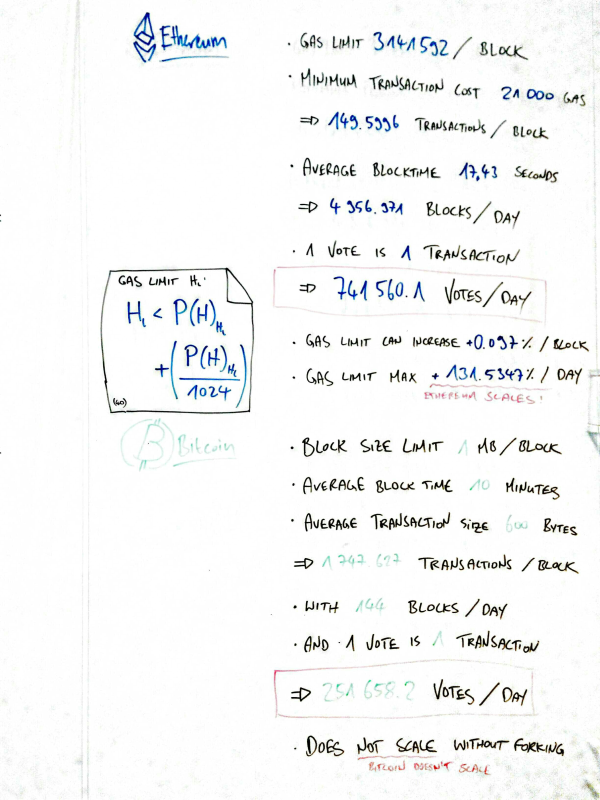
\includegraphics[draft,width=0.3\textwidth]{scale.png}
%\caption{scale.}
%\label{fig:scale}
%\end{figure}
Blockchain scalability is a hot debated topic right now. The Bitcoin blockchain has reached a state where almost each block in the network reached its maximum size of 1 MiB and on busy days the backlog of unconfirmed transactions piles up to several thousend transactions. The following scalability considerations will be made on a worst-case assumption which requires each vote to be a single signed transaction.
\subsubsection{Bitcoin scalability}
The Bitcoin block size limit is hardcoded at 1 MiB per block. The average block time is 10 minutes and the average transaction size to transfer funds is around 600 Bytes. This allows an average maximum of around 1748 transactions per block.
\begin{eqnarray}
& & \frac{1 \cdot 1024 \cdot 1024 B}{600 B} = 1747.62667 \frac {tx} {block}
\end{eqnarray}
With an average of 10 minutes per block there are 144 blocks per day.
\begin{eqnarray}
& & \frac{60 min \cdot 24 h}{10 \frac{min}{block}} = 144 \frac {blocks}{day}
\end{eqnarray}
With the assumption that one vote is one transaction and the blockchain is not used by anything else but voting, this allows roughly 251,659 votes per day.
\begin{eqnarray}
& & 144 \frac {blocks}{day} \cdot 1747.62667 \frac {tx} {block} = 251658.24 \frac{tx}{day}
\end{eqnarray}
Comparing that figure with numbers of registered voters in general elections around the world, one get's the idea what kind of limits this introduces. A big downside of Bitcoin is the unability to scale the number of transactions per time without introducing any network forks. Possible solutions exist but there is no consensus on which solution to use. Currently Bitcoin does \textit{not} scale.
\subsubsection{Ethereum scalability}
[SCHIENER~2015B] analyzed Ethereum blockchain voting and noticed that it would take around 40 days to hold the general elections of the United Kingdom on the Ethereum network. He gathered data from his own voting prototype which was not optimized regarding transaction size and also did not take into account that the block size is not fixed in Ethereum.\par
The Ethereum network determines fees by utilizing \textit{Gas}. Each transaction costs a certain amount of gas and each block has a block gas limit which determines the maxium of gas which can be spent each block. The current default gas limit of the Ethereum network after the Homestead release in March 2016 is 4,712,388 gas per block. The minimum cost of a transaction -- most likely just for transferring funds -- is 21,000 gas. This allows around 225 transactions per block by default.
\begin{eqnarray}
& & \frac {4712388 \frac{gas}{block}}{21000\frac{gas}{tx}} = 224.39943 \frac{tx}{block}
\end{eqnarray}
The current average block time is 15 seconds. Therefore, the network generates around 5760 blocks per day.
\begin{eqnarray}
& & \frac{60 min \cdot 24 h}{15 \frac{sec}{block}} = 5076 \frac {blocks}{day}
\end{eqnarray}
With the assumption that one vote is a transaction of minimal size and the network is not used for anything else, this allows to process 1,292,541 votes per day.
\begin{eqnarray}
& & 5076 \frac {blocks}{day} \cdot 224.39943 \frac {tx} {block} = 1292540.70857 \frac{tx}{day}
\end{eqnarray}\par
But that's only the default network capacity. Referring to the Ethereum yellow paper equations 44-46, the block gas limit scales as follows [WOOD~2014]:
\begin{eqnarray}
& & H_l < {P(H)_H}_l + \left\lfloor\frac{{P(H)_H}_l}{1024}\right\rfloor \quad \wedge \\ % 44
& & H_l > {P(H)_H}_l - \left\lfloor\frac{{P(H)_H}_l}{1024}\right\rfloor \quad \wedge \\ % 45
& & H_l \geqslant 125000 % 46
\end{eqnarray}
Simplyfied, this allows each block to grow by $1 + \frac{1}{1024}$ in terms of block gas limit. This allows a theoretic maximum increase of the block size limite by factor 142 per day.
\begin{eqnarray}
% & & \left( 4712388 \frac {gas}{block} + \frac{4712388 \frac {gas}{block}}{1024} \right) ^ {5076 \frac {blocks}{day}} = 141.82762
& & \left( 1 + \frac{1}{1024} \right) ^ {5076 \frac {blocks}{day}} = 141.82762
\end{eqnarray}
Ethereum scales by design only limited by physical boundaries like bandwith, available disk space and the central processing unit.
% [IMG: SCALABILITY-BTC-VS-ETH]

\subsection{Transaction fees issue}
%\begin{figure}[H]
%\centering
%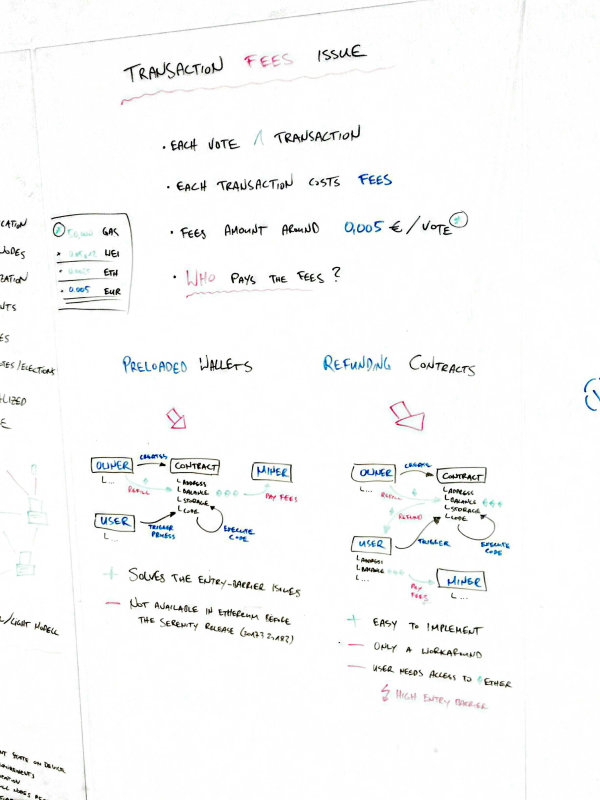
\includegraphics[draft,width=0.3\textwidth]{fees.png}
%\caption{fees.}
%\label{fig:fees}
%\end{figure}
Distributed ledgers are not controlled by anyone. Therefore, mechanisms have to be introduced which prevent spam or abuse of the network. Blockchain technology depends on fees which are usually paid by the signer of a transaction.\par
This introduces issues regarding several applications which operate on top of blockchains. Even though the fees are very low -- sometimes just a fraction of a cent -- they introduce an entry barrier for instance to interact with smart contracts or to vote on a blockchain.\par
Updating the records of the public ledger always costs fees. A fee worth less than a cent makes network attacks expensive but also requires every participant of the network to have access to the underlying currency. Decentralized applications must offer free transaction models to compete with centralized alternatives. Daniel Larimer of the Bitshares project adds, \enquote{it doesn't matter how good the service is, people expect certain things to be free} [LARIMER~2016].\par
Dominik Schiener calculated the average fees based on his proof-of-concept implementation would cost around 0.0091875 USD per vote [SCHIENER~2015B]. He further concluded, voting on blockchain is far cheaper compared to the costs of the general elections in the United Kingdom. However, any fee -- as low as it could ever be -- will just prevent a majority of potential users to use such applications.\par
A practical solution is still outstanding. Five approaches should be discussed for integration into future blockchain projects.
\subsubsection{Fractional reserve}
Larimer further suggests a dynamic fractional reserve which eliminates fees and introduces a model based on available \textit{bandwith} to write on the blockchain. The bandwidth is determined by how much stake (e.g., coins, gas) a participant in the network has [LARIMER~2016]. This is certainly a promising appraoch, but is still not free as users would have to hold any form of currency. This does not solve the underlying issue because it does not remove the initial entry barrier.
\subsubsection{Transaction server}
Schiener introduces a central polling server, which signes the transactions of the voters and pays the transaction fees [SCHIENER~2015A]. The fees are prefilled by the creator of the election. But this, however, introduces other issues, as discussed in section \ref{sec:pubv}.
\subsubsection{Refunding contracts}
Another approach could involve smart contracts refunding senders of transactions addressed at the contract. The creator of a poll fills the balance of the contract account and the user gets a refund after triggering the code execution on the contract based on his spent fees. This solution should be among the most easy ones to implement, however, it also does not remove the need to hold any unit of a crypto-currency. In addition, this might allow malicious parties to repeatedly call the contract to deplete its funds. % opens a door for spam or abuse of the network, as the user never faces any costs except the initial gas required to invoke the contract.
\subsubsection{Forwarding contracts}

%contract Gracious {
%  function runMe() {
%    this.realWork.gas(1000000)();
%  }
%}

\subsubsection{Contract pays}
The current model of most blockchain environments implements the earlier described \enquote*{sender pays} method where the signer of a transaction has to cover the fees. Recent advances in smart contract technology plan to implement new models.\par
Rootstock, which builds a smart contract platform on top of the Bitcoin platform, introduces an \enquote*{author pays}.
%One elegant blockchain implementation would offer the
%for some dapps, “contract pays” is a better model than “sender pays” as senders may not have any ether; now, individual dapps can implement such models, and if they are written in a way that miners can statically analyze and determine that they actually will get paid, then they can immediately accept them []

\subsection{Decentralized deadline consensus problem}
% decentralized deadline consensus problem: how to determine whether a message was sent before a certain deadline in a private, trustless, distributed system? [BORGSTRUP~2014]
% solution: dec cons deadl protocol [BORGSTRUP~2014]
% uses bitcoin nodes to create timestamps, costs fees [BORGSTRUP~2014]
% message interpretation layer on top of bitcoin timestamping, which handles msgs as votes [BORGSTRUP~2014]

\subsection{Voting coercion in distributed systems}
% possibility of revoting against coercion [BORGSTRUP~2014]

% steps of voting are transactions on the blockchain [HOURT~2015B]
% id verification -> transaction [HOURT~2015B]
% each id voted at most once [HOURT~2015B]
% broadcast new transaction for each decision change

% revoting: chaining votes with previous trx hashes [BORGSTRUP~2014]

\subsection{Power distribution with proof-of-work}
% pow, pos lottery
% a+b > 51%
% disruption of processing
% possible solution federated transaction consensus
% equal distribution of power, control

\section{Outlook}
% todo

\section{License}
This paper is available in the public domain (CC0).

\section{Further Reading}
[BALE~2014] Bale, A (2014): BitVote, Vote With Your Live, Whitepaper, 11 June~2014, Louisville, Kentucky, United States of America.\par
[BORGSTRUP~2014] Borgstrup, J (2014): Private, Trustless And Decentralized Message Consensus And Voting Schemes, Master's Thesis, 23~November~2014, University of Copenhagen, Denmark.\par
[BUTERIN~2014] Buterin, V (2014): A Next-Generation Smart Contract And Decentralized Application Platform, Ethereum Whitepaper, 11~January~2014, Ethereum Project: http://vbuterin.com/ethereum.html\par
[BUTERIN~2015] Buterin, V (2015): Understanding Serenity, Part I: Abstraction, Ethereum Blog, 24~December~2015, Canada.\par
[COYNE~2015] Cyone, C (2015): New Voting System Proposed For~2016 SGA Elections, The Daily Athenaeum, 19~November~2015, Morgantown, West Virginia, United States of America.\par
[DEMOCRACYOS~2015A] Anonymous (2015): Blockchain support for DemocracyOS, DemocracyOS Blog, 19~March~2015, Buenos Aires, Argentina.\par
[DEMOCRACYOS~2015B] Anonymous (2015): Why blockchain support for DemocracyOS, DemocracyOS Blog, 24 June~2015, Buenos Aires, Argentina.\par
[ELVIRA~2013] Elvira, ER (2013): A Bitcoin Based, Completely Distributed Voting System, 28~November~2013, Agora Voting Blog, Madrid, Spain.\par
[ÉPIÉ~et~al.~2015] Épié, C; Loubet, N (2015): Blockchain and Beyond, Version 1.0, 3~December~2015, Cellabz, Paris, France.\par
[ERFURT~2015] Erfurt, D (2015): Ein dezentrales Transitionssystem zur Manipulation von geteilten Wörtern einer regulären Sprache, Bachelor's Thesis, 25 June 2015, Humboldt University, Berlin, Germany.\par
[ERFURT~2016] Erfurt, D (2016): Efficient Decentral Governance of Structured Data, Whitepaper, 21~March~2016, Berlin, Germany: http://memhub.io/whitepaper\par
[ERNEST~2014] Ernest, AK (2014): The Key To Unlocking The Black Box: Why The World Needs A Transparent Voting DAC, 4~July~2014, Follow My Vote, Blacksburg, Virginia, United States of America.\par
[ERNEST~2016] Ernest, AK (2016): Follow My Vote, 26~January~2016, In: Report On Secure Voting, A Guide To Secure \#onlinevoting In Elections, Webroots Democracy, United Kingdom.\par
[HOURT~2015A] Hourt, N (2015): End to End Verified Voting On A Blockchain, 3~September~2015, Follow My Vote, Youtube: https://youtu.be/EE2mWoio7po\par
[HOURT~2015B] Hourt, N (2015): How Our Voter Registration Process Works, 16~December~2015, Follow My Vote, Youtube: https://youtu.be/GcAz9mZW1\_c\par
[JOHNSTON~et~al.~2013] Johnston, DA; Yilmas, SO; Kandah, J; Bentenitis, N; Hashemi, F; Gross, R; Wilkinson S; Mason, S (2013): The Generalized Theory Of Decentralized Applications, DApps,~20~November~2013, DAppsFund, Austin, Texas, United States of America.\par
[KAYE~2014] Kaye, M (2014): A First Attempt To Describe The Neutral Voting Bloc, 2~July~2014, VoteFlux, Sydney, Australia.\par
[KAYE~2016] Kaye, M (2016): Public VoteFlux Slack Channel Archive (\#general), 12~March~2016, VoteFlux, Sydney, Australia.\par
[KONASHEVYCH~2016] Konashevych, O (2016): What Are We Doing, 25~February~2016, E-Vox.org, Kiev, Ukraine.\par
[LARIMER~2016] Larimer, D (2016): How To Build A Decentralized Application Without Fees, 10~February~2016, Bitshares, Blacksburg, Virginia, United States of America.\par
[LEVEL~2014] Level, C (2014): VoteCoin, A fair, transparent, practical solution to fix modern voting, VoteCoin Blog, 9~December~2014, United States of America.\par
[MANCINI~2015] Mancini, P (2015): Blockchain Support For Open Source Platform Democracyos, Newschallenge, 17~March~2015, San Francisco, California, United States of America.\par
[MANCINI~et~al.~2015] Mancini, P; Siri, S (2015): Democracy Earth, Power In Your Hands, A Decentralized Global Commons Of Peers, San Francisco, California, United States of America.\par
[MARGOT-DUCLOT~2015] Margot-Duclot, L (2015): Nemos, Whitepaper, 2015, Paris, France.
[MONEGRO~2014] Monegro, J (2014): The Blockchain Application Stack, 25~November~2014, Union Square Ventures, New York, United States of America.\par
[NAKAMOTO~2008] Nakamoto, S (2008): Bitcoin, A Peer-to-Peer Electronic Cash System, Bitcoin Whitepaper, 31~October~2008, Metzdowd Cryptography Mailing List: https://bitcoin.org/bitcoin.pdf\par
[NOIZAT~2014] Noizat, P (2014): Blockchain Electronic Vote, Unchain.Voting Whitepaper, 30~July~2014, Paymium, Paris, France.\par
[ROCKWELL~2014] Rockcoons \enquote{Rockwell}, M (2014): BitCongress, Whitepaper, Blockchain Based Voting System, 16~October~2014, Bitcoin Kinetics, Beaverton, Oregon, United States of America.\par
[SCHIENER~2015A] Schiener, D (2015): Public Votes, Ethereum-based Voting Application, 28~October~2015, South Tyrol, Italy.\par
[SCHIENER~2015B] Schiener, D (2015): Voting on the Ethereum Blockchain, An Analysis, 7~November~2015, South Tyrol, Italy.\par
[SCOTT~2016] Scott, B (2016): How Can Cryptocurrency And Blockchain Technology Play A Role In Building Social And Solidarity Finance, Working Paper~2016-1, 25~February~2016, United Nations Research Institute for Social Development, Geneva, Switzerland.\par
[VARSHNEYA~et~al.~2015] Varshneye, AJ; Poudel, S; Vyas, X (2015): Blockchain Voting, CS4501 Cryptocurrency Cabal, 7~December~2015, University of Virginia, United States of America.\par
[WOOD~2014] Wood, G (2014): Ethereum, A Secure Decentralised Generalised Transaction Ledger, Ethereum Yellowpaper, 6~April~2014, Ethereum Project: http://gavwood.com/paper.pdf

% @TODO refs nemos io

\end{multicols}
\end{document}
